\section{Online renderelő}
\rhead{Online renderelő}
\label{raytracer}

Az épületek bemutatásának elősegítése érdekében szerettünk volna egy valósághű képalkotó programot létrehozni, amely beépül a honlapba és a szerkesztőbe is. Erre a célra egy hálózaton elosztott path tracer-t írtunk a Rust nevű programozásnyelvben.

\subsection{Raytracer}
Az elmúlt pár évben kifejezetten felkapott lett a \emph{Raytracing} kifejezés. Ezt az Nvidia RTX videokártyáinak megjelenése segítette elő, hiszen ez az első olyan eszköz, amely képes ezt a folyamatot valós idejűleg megcsinálni.

A raytracing egy módszer három dimenziós jelenetek két dimenziós képekké alakítására a valós fizika szabályain alapuló módszerekkel. Egy másik gyakran használt módszer a raszterizálás, amit általában a játékok és más valós idejű szoftverek (például az Archytex szerkesztő) használnak, mert gyorsabb, de nem olyan sokoldalú és valósághű, mint a raytracing.


\subsubsection{A módszer leírása}
A raytracing lényege, hogy a kamera képének minden egyes pixeléből egy-egy sugarat "lövünk" ki és megnézzük, hova landol. Landolás után a sugárhoz tartozó pixelt a landolás helye és az ott lévő felület szerint beszínezzük.

E szerint három fő komponense van egy ilyen rendszernek: egy kamera, egy módszer a sugarak landolási helyének megállapítására és egy módszer a pixelek beszínezésére. A raytracer-ek sokoldalúsága abból adódik, hogy sokféle komponens létezik, amely ezeket a feladatokat felveheti. Teljesen árnyékmentes, csak gömbökkel foglalkozó lyukkamerát használó megoldásoktól kezdve egészen a valósággal összehasonlíthatatlan képeket generáló megoldásokig mindenre képes a megfelelő komponensekkel.

\begin{figure}[H]
    \centering
    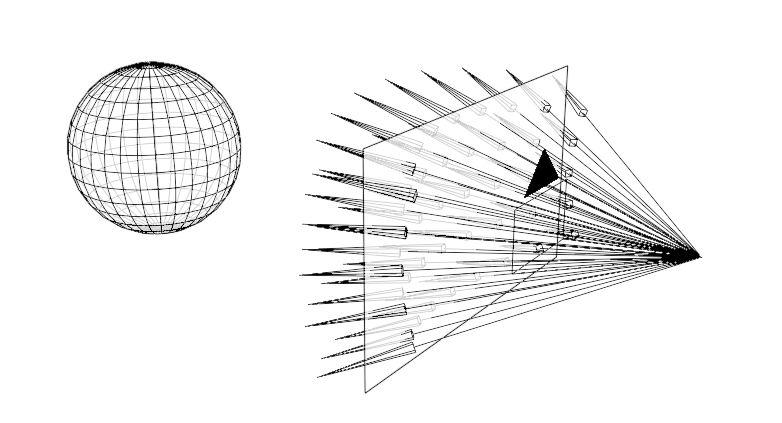
\includegraphics[width=0.5\textwidth]{parts/developer-documentation/ray-tracer/images/figure.png}
    \caption{A Raytracer működési elve}
\end{figure}
\subsubsection{Gyorsító struktúrák}

A fent említett három komponens közül a a sugár landolásának megkeresése jár a legnagyobb számítási költséggel, hiszen ezt pixelenként kell megnézni, akár többször is.

Az Archytex-ben háromszögekből álló modellekkel dolgozunk. Ha a gép meg szeretné tudni, hogy egy sugár hol találkozik a modell akármelyik részével, akkor mindegyik háromszöget egyenként meg kell nézni. Ez egy összetettebb épület esetén megtöbbszörözheti a feldolgozási időt.

Ennek az időnek a lecsökkentésére különböző gyorsító struktúrákat használhatunk. Manapság a leggyakoribb ilyen struktúra a Bounding Volume Hierarchy (BVH).

A BVH lényege, hogy minden háromszöghöz hozzárendelünk egy téglatestet (1. szint), amelybe belefér, majd az egymás mellett lévő téglatesteket párokba helyezzük és azokat is téglatestekbe helyezzük (2. szint). Ezt addig folytatjuk, amíg végül csak egy téglatest marad hátra.

A sugarak feldolgozásakor először leellenőrizzük, hogy eltalálja-e a külső téglatestet. Ha nem találja el, akkor a háromszögek közül sem találhatta el egyiket se. Ha a téglatestet eltalálta, akkor az abban lévő téglatestekkel is meg kell tennünk ugyan ezt az ellenőrzést. Ennek az előnye, hogy átlagosan az algoritmus komplexitása $O(n)$-ről $O(log(n))$-re csökkent.

\subsection{Rust}
A renderelő rendszer elkészítéséhez Rust-ot használtunk. Ennek több oka is van:

Mint a szerkesztőnél, itt is fontos szempont volt a gyorsaság, hiszen minél kevesebb önköltsége van a programozási nyelvnek, annál gyorsabb algoritmusokat lehet írni.

Ezzel szemben lényeges a biztonság is. A C és a C++ gyors, rendszerközeli nyelvek, de nem érkeznek ugyanazokkal a biztonsági garanciákkal, mint a Rust. Ez nem előnyös egy online renderelő esetén, hiszen a felhasználótól kéri az adatokat, és olyan környezetben fut, ahol el lehet érni bizalmas adatokat. C és C++ esetén bizonyos programhibákkal egy támadó képes átvenni az irányítást a szerver felett, és más felhasználók adatait ellopni.

Fontos még kiemelni a Rust generikus rendszerét, amely elősegíti a fent említett komponensek szétválasztását és egybeágyazását különféle compile idejű optimalizációkkal.

\subsection{Path tracer}
A raytracer-ek segítségével lehet a fény viselkedését is szimulálni. Ezt hívjuk path trace-nek.

Lényege, hogy a kamerából kiinduló sugaraknak hagyjuk, hogy a felületre érkezve folytassák útjukat egy másik irányba. Ez az irány a felület tulajdonságaitól függ. Egy tükör a sugarat csak egy irányba küldheti tovább, míg egy téglafal a fényt szórja, tehát több lehetséges iránya is van a fénynek.

A helyes megjelenítéshez a lehetséges irányok terén kell integrálni az egyes irányokhoz tartozó értékeket az adott irány szerint súlyozva. Ez egy olyan integrálási probléma, amelynek nincs tényleges megoldása, csak megközelíteni tudjuk.

Erre a megközelítésre létezik a Monte Carlo integrálás. Lényege, hogy a lehetséges irányok közül egy megadott darabot (sample szám) kiválasztunk véletlenszerűen, majd azokat átlagoljuk.

Az így keletkezett kép a várt képnek csak egy megközelítése. Minősége a sample számtól függ. Alacsony sample szám esetén a kép zajos lehet, magas sample szám esetén a feldolgozás ideje megnőhet.

\begin{figure}[H]
    \centering
    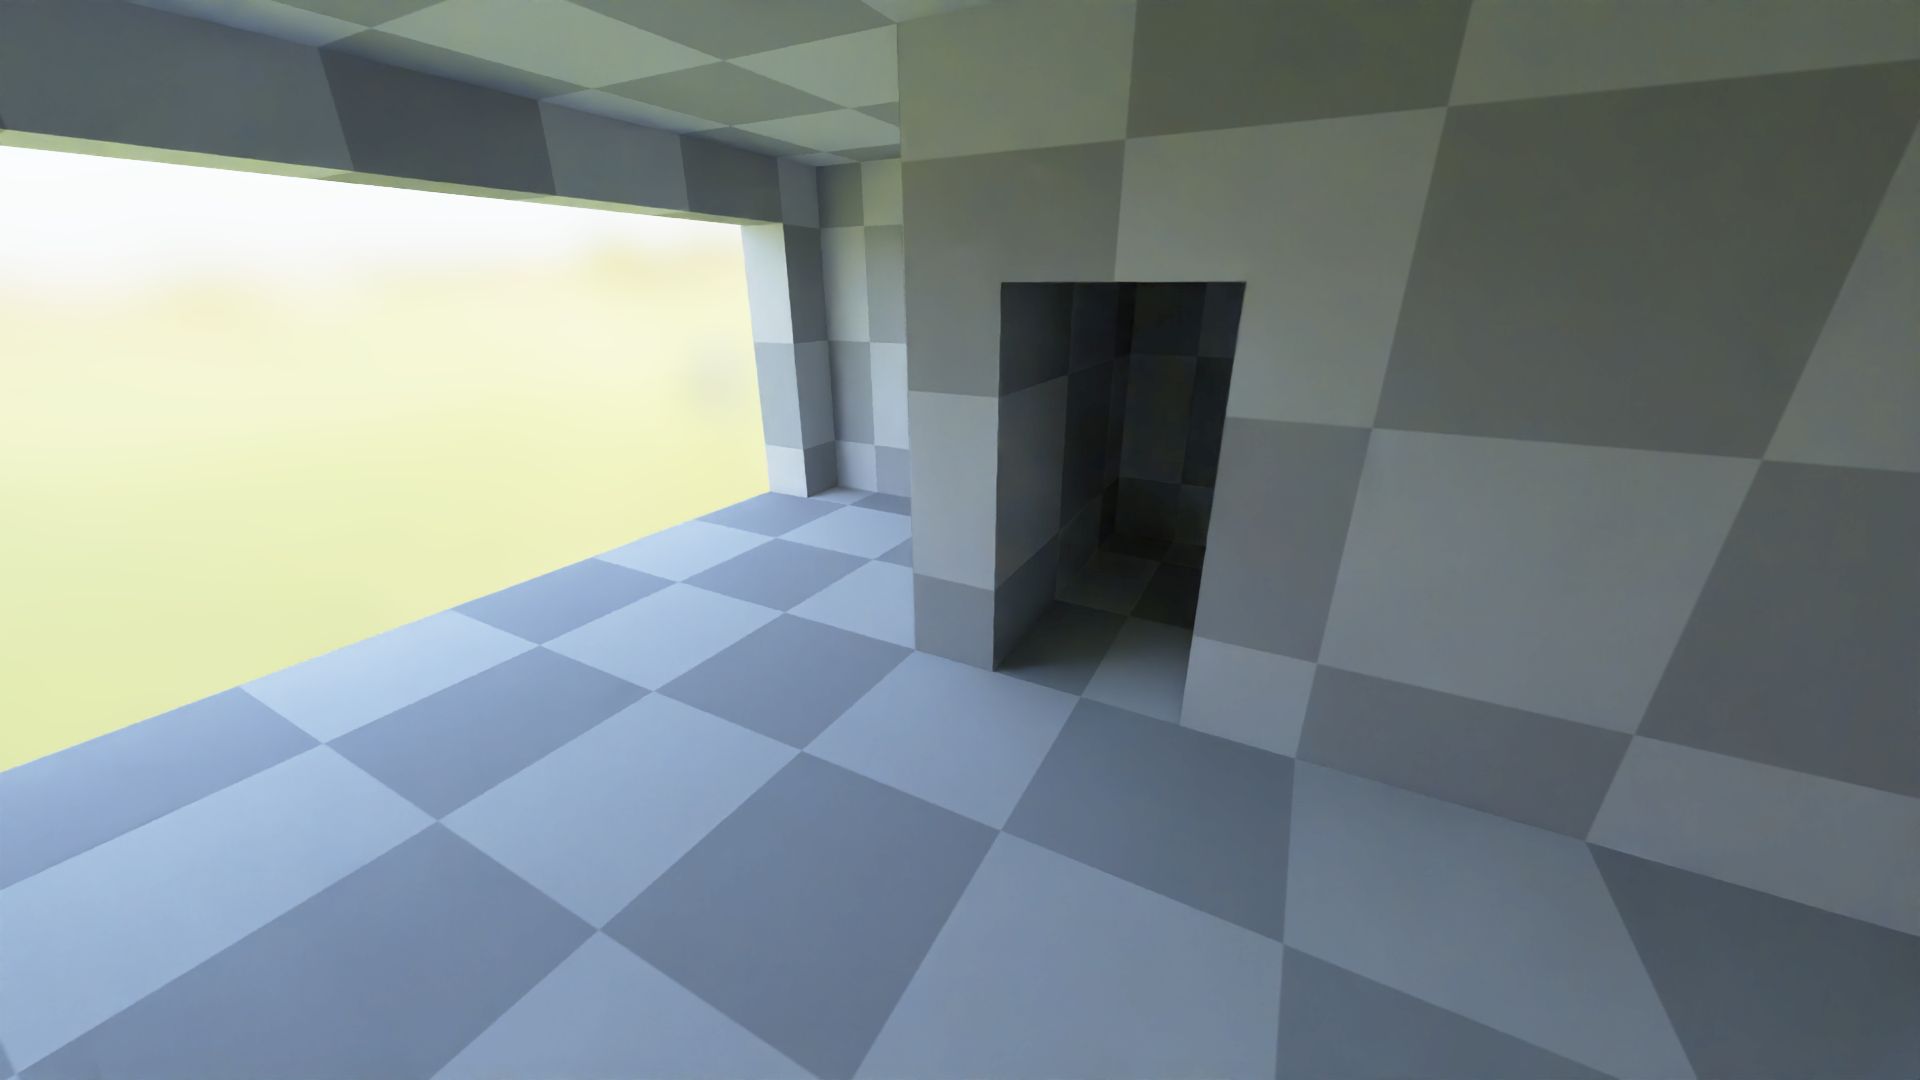
\includegraphics[width=0.5\textwidth]{parts/developer-documentation/ray-tracer/images/example.png}
    \caption{Példa, a Path Tracer által létrehozható képekre}
\end{figure}

\subsubsection{Open Image Denoise}
Hogy alacsony sample szám esetén is viszonylag jó minőségű képeket kapjunk, az Intel által fejlesztett Open Image Denoise\footnote{\url{https://www.openimagedenoise.org/}} nevű szoftvert használjuk.

Ez a szoftver mesterséges intelligenciát használ a képen lévő zaj eltávolítására.

Csak x86 alapú rendszereken elérhető.

\begin{figure}[H]
    \centering
    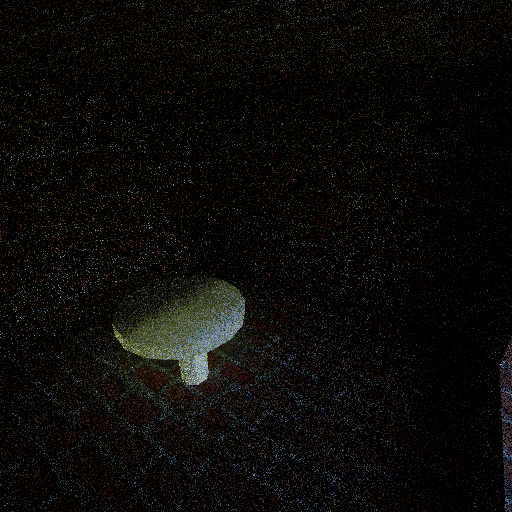
\includegraphics[width=0.25\textwidth]{parts/developer-documentation/ray-tracer/images/raw.png}
    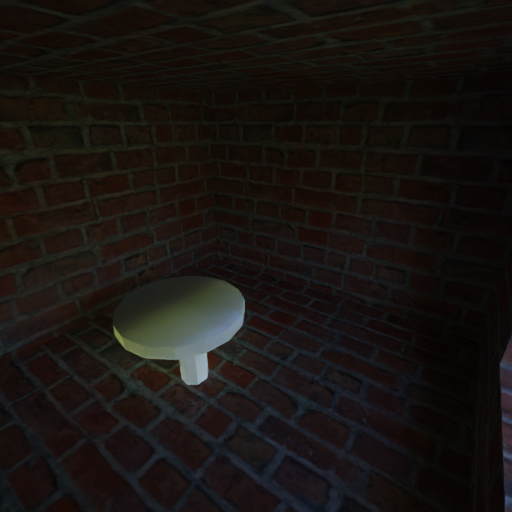
\includegraphics[width=0.25\textwidth]{parts/developer-documentation/ray-tracer/images/denoised.png}
    \caption{Összehasonlítás a nyers (bal) és a zajszűrt (jobb) képek között}
\end{figure}

\subsection{Elosztott renderelő}

A képek elkészítési idejének csökkentésére a renderelőhöz hozzáadtunk egy elosztási rendszert.

Ez a rendszer RabbitMQ-ra\footnote{\url{https://www.rabbitmq.com/}} és Redis-re\footnote{\url{https://redis.io/}} épül. A RabbitMQ egy üzenetküldő rendszer, amely a különböző rétegek közti kommunikációt segíti elő, míg a Redis egy kulcs-érték adatbázis a hosszabb ideig szükséges és nagyobb adatok tárolására.

A Redis szerverhez hozzáadtuk a RedisAI\footnote{\url{https://oss.redis.com/redisai/}} kiegészítőt, amivel lehet tömbökön végrehajtani matematikai operációkat. Ez a későbbiekben még hasznos lesz.

Az egyszerűbb kezelés érdekében, két különböző réteget hoztunk létre: a tartomány kezelő réteg (domain manager) és a feliratkozó réteg (subscriber)

\subsubsection{Tartománykezelő réteg}
A Tartománykezelő réteg feladata a renderelési kérések fogadása a backendtől, majd ezen kérések munkákra osztása és összerakása.

A renderelés elkezdéséhez egy véletlenszerű azonosítót kell generálnunk a kérésünk számára (ID) és Redis-ben a következő értékeket kell beállítanunk:

\begin{itemize}
    \item archyrt:ID:width

          A várt kép szélessége pixelben
    \item archyrt:ID:height

          A várt kép magassága pixelben
    \item archyrt:ID:samples

          A renderelés során használt sample-ök száma
    \item archyrt:ID:scene

          A projekt által használt .ascn bináris fájl
\end{itemize}

A kéréseket a RabbitMQ \emph{archyrt:dispatch} sorából várja. Az innen beérkező üzenetek karakterláncok, amelynek formátuma:

\begin{figure}[H]
    \centering
    \begin{minipage}{.7\textwidth}
        \begin{lstlisting}
keresID#felhasznaloID#projektID
\end{lstlisting}
    \end{minipage}
\end{figure}

Ekkor a tartománykezelő a képet felosztja 16 egyenlő részre (csempe), és minden rész minden egyes sample-jéhez egy-egy munkát köt a saját egyedi azonosítójával. A munkákat a \emph{archyrt:taskqueue} sorba küldi a következő formátummal:

\begin{figure}[H]
    \centering
    \begin{minipage}{.7\textwidth}
        \begin{lstlisting}
keresID#munkaID#visszateresiSorNeve#csempeXKoordinataja#csempeYKoordinataja
        \end{lstlisting}
    \end{minipage}
\end{figure}


A fenti üzenetben megadott sorból egyenként elfogadja az üzeneteket, az üzenetből kiolvassa, hogy a munka során generált kép hova lett mentve, és feldolgozza azt.

\begin{figure}[H]
    \centering
    \begin{minipage}{.7\textwidth}
        \begin{lstlisting}
RedisKulcsAholAKepVan#CsempeX#CsempeY
        \end{lstlisting}
    \end{minipage}
\end{figure}

Ezek után a tartománykezelő végrehajtja a zajeltávolítást, és elmenti a képet a fájlrendszerbe.

\subsubsection{Feliratkozó réteg}
A feliratkozó réteg feladata a Tartománykezelő által kiadott munkák végrehajtása.

Miután megkapta a feladatot az \emph{archyrt:taskqueue} sorból (lásd fent), betölti a Redis-ből a kéréshez tartozó jelenetet, és kirendereli azt. Renderelés után feltölti Redis adatbázisba tenzorként, véletlenszerű kulccsal és ezt jelzi a tartománykezelőnek.